%===================================
%===================================
%===================================
\setchapterpreamble[u]{\margintoc}
\chapter{Combined cooling pilot plant at Plataforma Solar de Almería}
\labch{cc:facility}

\tldrbox{
    In this chapter a detailed description of the combined cooling pilot plant
    at \gls{psaLabel} is provided including a \gls{pYidLabel} diagram and the
    methodology followed to perform the experimentation and data-processing.
    Three experimental campaigns for the \gls{wctLabel} with XX, XX and XX
    different operating points and one for the \gls{dcLabel} with XX operating
    points are processed and made openly available in public repositories.
}

\section*{Introduction}

The combined cooling pilot plant at Plataforma Solar de Almería is a unique
facility that integrates a wet cooling tower and a dry cooler in a flexible
hydraulic configuration. It allows for the study and validation of different
cooling strategies and the development of models. \todo{completar esta sección antes del domingo}

% Historia de la planta
...

This chapter describes the
plant in \nrefsec{cc:facility:description} and the experimental campaigns carried
out in \nrefsec{cc:facility:exp}.

% TODO: A la salida de la segunda válvula hay que añadir una flecha para que
% sea más legible, renombrar válvulas V1 y V2 a Vp y Vs.
\begin{figure*}[h!]
	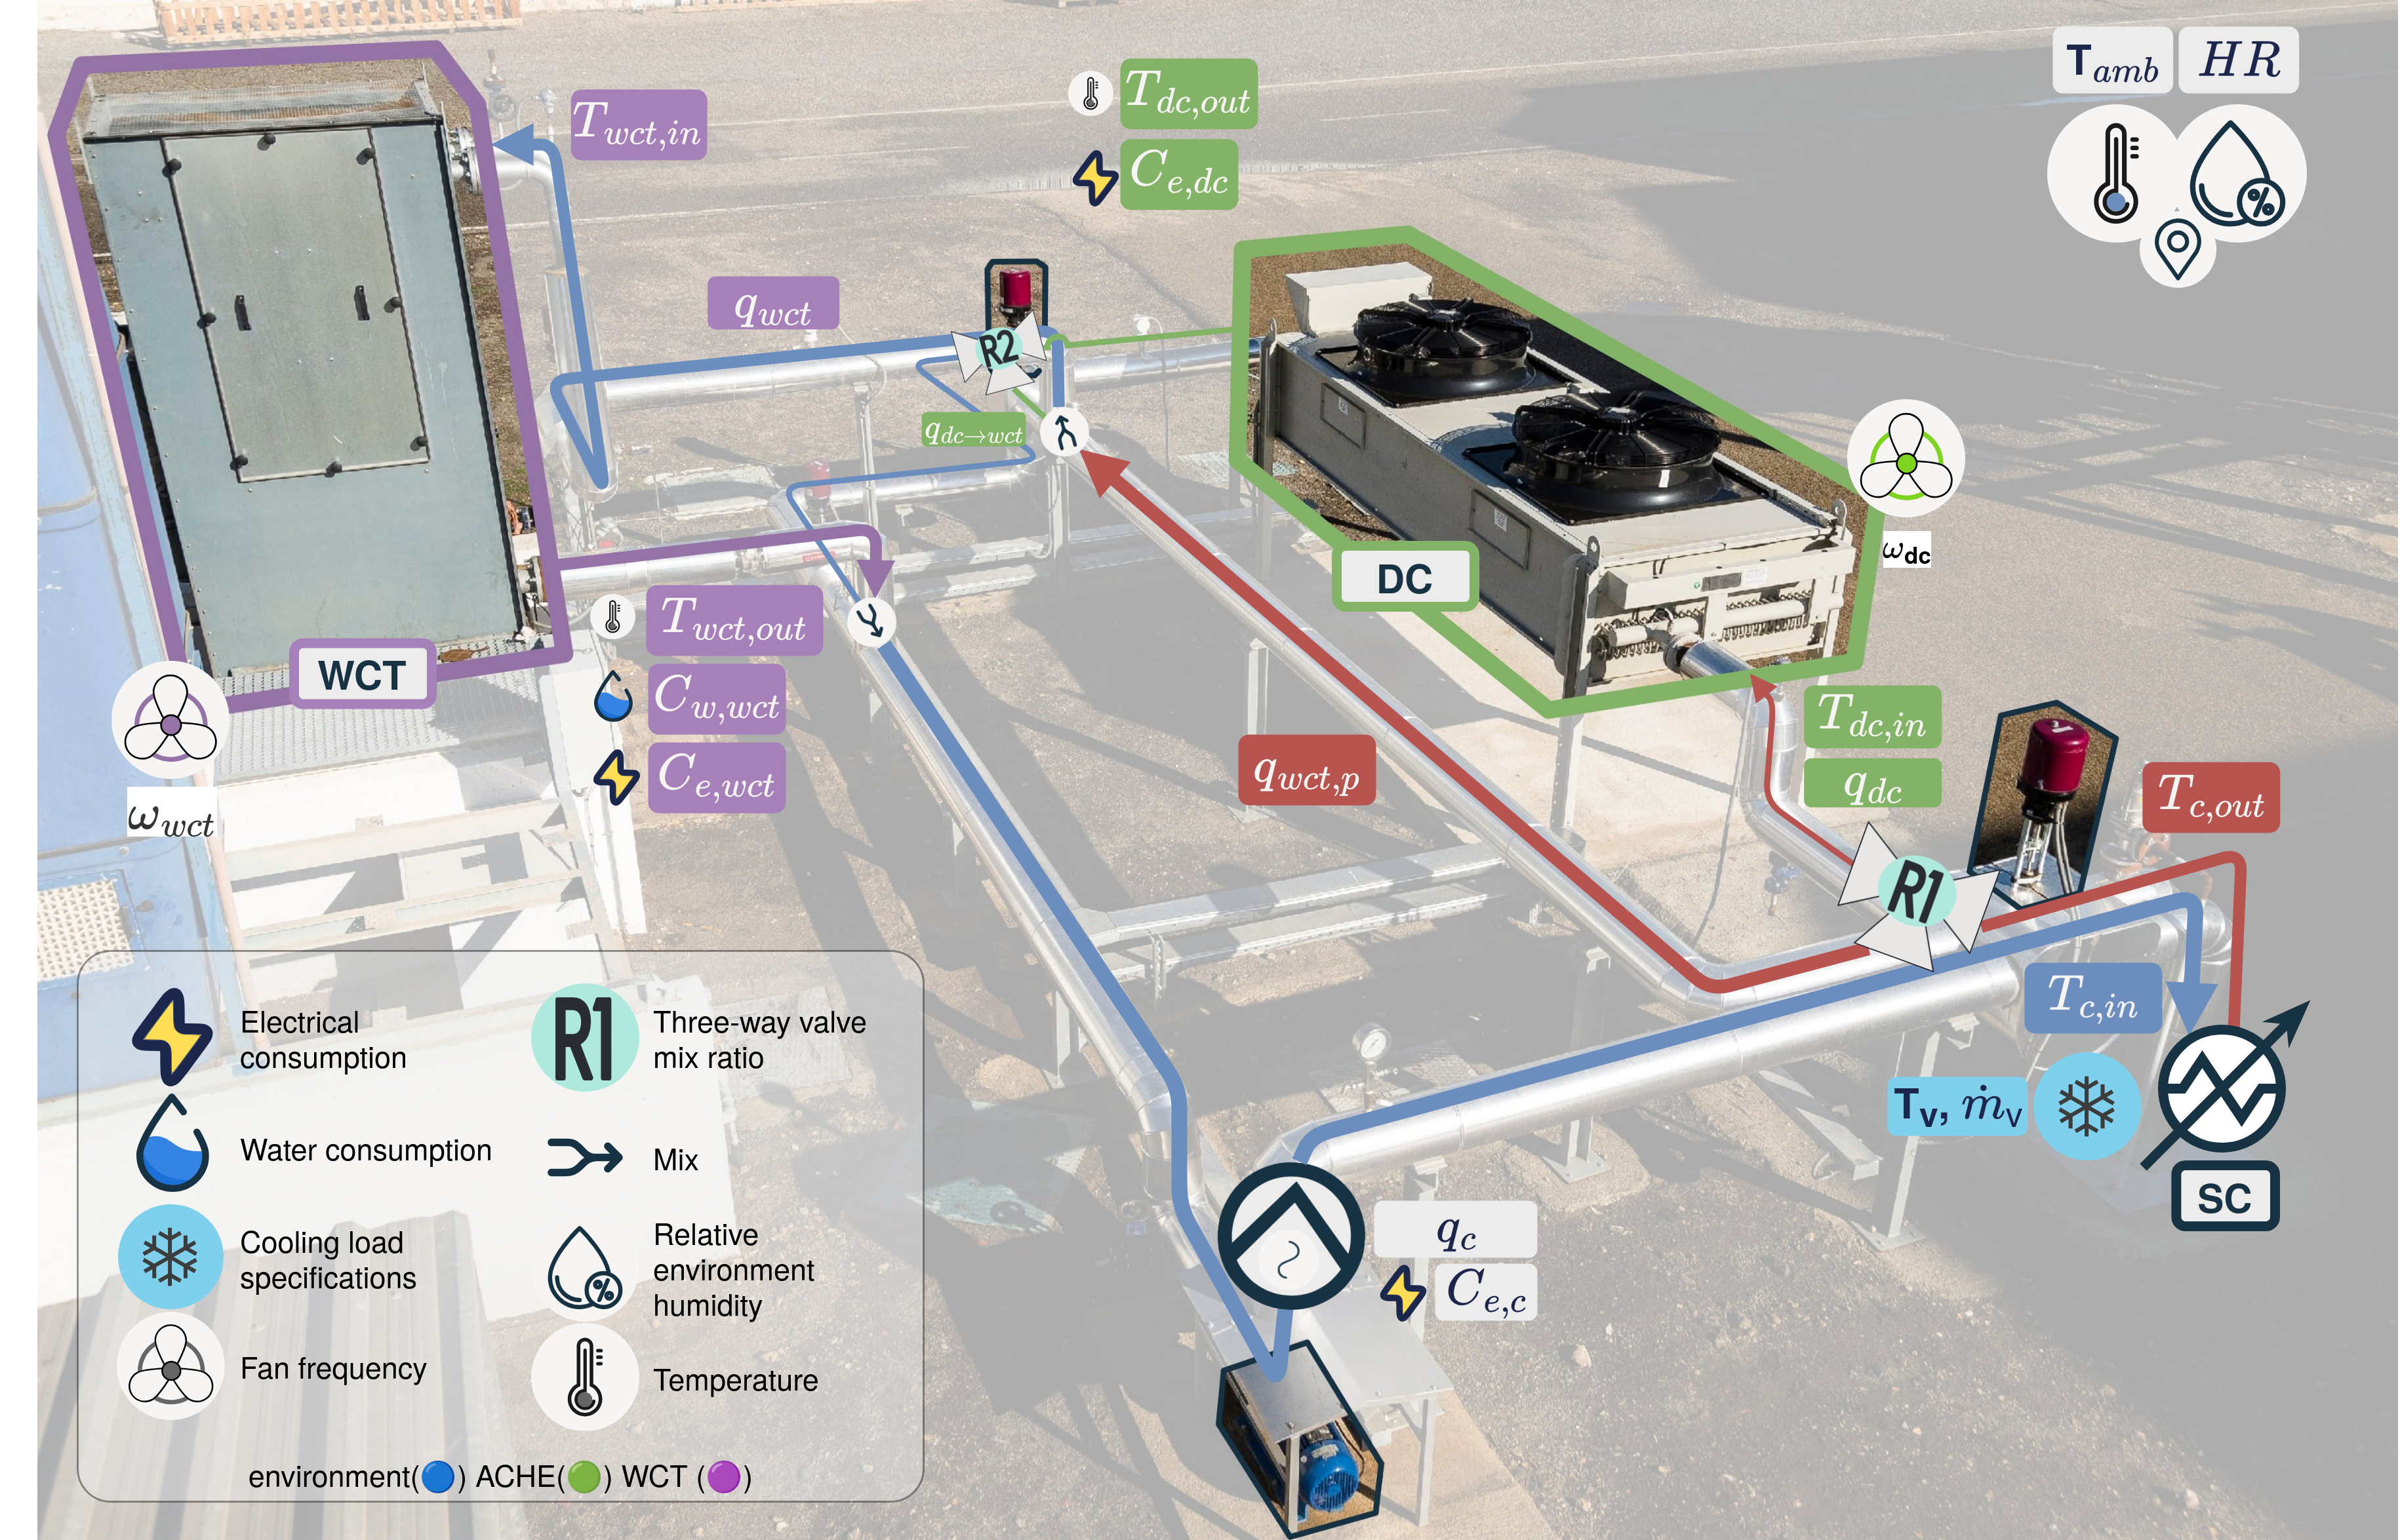
\includegraphics[]{figures/WASCOP-facility-diagram.png}
	\caption{\gls{psaLabel} combined cooling system facility}
	\labfig{cc:facility:cc-pilot-plant-diagram}
\end{figure*}


%===================================
%===================================
\section{Plant description}
\labsec{cc:facility:description}

% TODO: Aquí habría que añadir una figura estilo diagrama de bloques, que no
% incluya solo el circuito de refrigeración, sino también los circuitos de
% intercambio y generación de calor.

% The combined cooling pilot plant at the Plataforma Solar de Almería consists of three
% circuits: cooling circuit, exchange circuit and heating circuit. In the cooling
% circuit (shown in
% Figure \reffig{cc:facility:cc-pilot-plant-diagram}), water circulating inside the tube bundle of a surface condenser is
% cooled through a \gls{wctLabel} and/or a \gls{dcLabel} of the \gls{acheLabel}
% type. Valves 1 and 2 (R$_p$, R$_s$, respectively) allow operation in different
% configurations: \gls{dcLabel} only, \gls{wctLabel} only, in series, in parallel
% with different opening percentages, or parallel-series. In the exchange
% circuit, a saturated steam generator generates steam at different pressures,
% which is in turn condensed through the Surface Condenser, transferring its
% latent heat to the cooling water that is thus heated. Finally, in the heating
% circuit, a static solar field provides the thermal energy required by the steam
% generator using hot water as heat transfer fluid. A more detailed description
% of this installation can be found in Palenzuela et
% al.~\cite{palenzuela_experimental_2022}.

% Sacado de: Wet cooling tower performance prediction in \gls{cspLabel} plants:
% A comparison between artificial neural networks and Poppe’s model
The pilot plant of combined cooling systems located at \gls{psaLabel} (see the
layout in \reffig{cc:facility:pid}) consists of three circuits:
cooling, exchange and heating. In the cooling circuit (see a picture in
\reffig{cc:facility:wct-back-view}), water circulating inside the tube bundle of
a Surface Condenser (SC) can be cooled through a Wet Cooling Tower and/or a Dry
Cooling Tower (type Air Cooled Heat Exchanger, ACHE), both with a designed
thermal power of 204~kW$_{th}$. In the exchange circuit, a saturated steam
generator of 80~kW$_{th}$ (on the design point), generates steam at different
pressures (in the range between 82~mbar and 200~mbar), which is in turn
condensed in the surface condenser. In this way, the steam transfers its latent
heat of condensation to the refrigeration water, that is heated. Finally, in
the heating circuit, a solar field with a thermal power of 300~kW$_{th}$ at the
design point, provides the energy required by the steam generator, in the form
of hot water. It is a unique, very flexible, fully instrumented and versatile
facility, able to operate in different operation modes: series and parallel
mode, conventional dry-only mode (all water flow is cooled through the dry
cooling tower) and wet-only mode (all water flow is cooled through the wet
cooling tower). The instrumentation related to the WCT is described in Table
\reftab{cc:facility:instr}. Note that the sensors measuring the air
velocity and temperature and relative humidity at the outlet area of the wet
cooling tower have not been installed in the plant. Portable sensors were used
instead in some experiments, as described in Section \ref{sec:Data1}.

\begin{marginfigure}[-7cm]
    \includegraphics[]{figures/WASCOP-facility-WCT.png}
    % \caption{Back view of the WCT}
    \savebox\captionqr{\qrcode[hyperlink,height=0.4in]{\repositoryBaseUrl/figures/day_viz_20220614_eval_at_20250414T1247_test_water_price.html}}
	\caption[Back view of the WCT]{Back view of the
	WCT.\hspace{1ex}\usebox\captionqr}
    \labfig{cc:facility:wct-back-view}
\end{marginfigure}

In regards to operational aspects of the system, note that the cooling water
and air flow rates at the experimental facility ($\dot{m}_w$, and air,
$\dot{m}_a$, respectively), are modified with the \textit{Pump 1} and the fan
frequency percentage \texttt{SC-001}, respectively (see
\reffig{cc:facility:pid}).

\begin{table}[h]
\caption{Characteristics of instrumentation ($^a$ value of the temperature in $^\circ$C, $^b$ of reading, $^c$ full scale, $^d$ mean value).} 
\labtab{cc:facility:instr}
\resizebox{\linewidth}{!}{
\begin{tabular}{cccc} 
    \toprule
    \textbf{Measured variable} & \textbf{Instrument} & \textbf{Range}  &
    \textbf{Measurement uncertainty}\\
    \midrule
    Water temperature & Pt100 & 0 - 100 $^\circ$C & 0.03 + 0.005$\cdot T^a$\\
    (\texttt{TT-001}, \texttt{TT-006}) & & &\\
    Cooling water flow rate & Vortex flow meter & 9.8 - 25 m$^3$/h & $\pm$ 0.65
    \% o.r.$^b$\\
    (\texttt{FT-001})  & & &\\
    Water flow rate  & Paddle wheel & 0.05 - 2 m$^3$/h & $\pm$ 0.5 \% of
    F.S$^c$  \\
    (\texttt{FT-004}) & flow meter  & & + 2.5 \% o.r\\
    Ambient temperature & Pt1000 & -40 - 60 $^\circ$C  & $\pm$ 0.4 $@$20
    $^\circ$C \\
    Relative humidity & Capacitive sensor & 0 - 98\% & $\pm$ 3 \% o.r $@$20
    $^\circ$C  \\
            Air velocity & Impeller anemometer & 0.1-15$~\mbox{m s$^{-1}$}$ &
            $\pm$ 0.1$~\mbox{m s$^{-1}$}$ + 1.5 \%  o.r \\
            Outlet air temperature & Pt100   & -20-70$^\circ$C & $\pm
            0.5^\circ$C \\
            Outlet air humidity & Capacitive sensor   & 0-100\%& $\pm$ 2\% \\
    \bottomrule
\end{tabular}
}
\end{table}

\begin{figure}
    \includegraphics[width=1\textwidth]{figures/WASCOP-facility-PID.png}
    \caption{Layout of combined cooling systems pilot plant at \gls{psaLabel}.}
    \labfig{cc:facility:pid}
\end{figure}


%===================================
%===================================
\section{Experimental campaigns}
\labsec{cc:facility:exp}

With the aim of characterizing and developing models for this novel facility,
over the years several experimental campaigns have been carried out. In
particular, three different experimental campaigns have been performed to
characterize the \gls{wctLabel} specifically, while a campaign was also carried
out to characterize the \gls{dcLabel}.

\section[Experimental campaigns for the wet cooling tower]{Experimental campaigns for the wet cooling tower}[Wet cooling tower]
\labsec{cc:facility:exp-wct}

A total of 132 steady-state experimental points have been obtained. These data
cover a large variety of ambient conditions (different seasons, days and
nights) and thermal loads (from 27 kW to 207 kW). The objective of the
experimental campaigns is to develop and validate two modelling strategies for
the performance evaluation of the \gls{wctLabel}\sidenote{See
\nrefsec{cc:modelling:wct}}.

The normative framework followed to carry out the
experiments, in order to ensure stable conditions, has been the standards
\texttt{UNE 13741}~\sidecite{une_thermal_2004a}
%\sidenote{\textit{Thermal Performance Acceptance Testing of Mechanical Draught
%Series Wet Cooling Towers} },
and the Spanish CTI~\sidecite{cti_code_2000}. These standards specify the test
duration and the allowed variations of the most representative ambient and
operating magnitudes (water flow rate, heat load, cooling tower range,
wet-bulb and dry-bulb temperatures and wind velocity) during the tests.
Although the duration of the test should not be less than one hour according
to the standards, due to the low capacity of the WCT in the PSA pilot plant
and the operational experience, the duration of the tests has been reduced to
up to 30 minutes. Once stable conditions are maintained during the defined
interval time, the average and deviations values of each measurement are
calculated in order to check that they are within the allowable limits of the
norm, which finally lead to a valid steady-state operating point. 

\reffig{cc:facility:example-test} shows the main variables involved in one of
the experiments performed at the pilot plant at constant air flow rate
($f_{fan}$=25~\%). As can be observed, there are two time intervals in this
case, in which the process is at stationary conditions according to the
normative framework mentioned. In order to process the results of the
experimental tests and identify valid time intervals, such as the ones shown in
this example, a function has been implemented in the \textit{MATLAB}
environment. This function identifies whether the standard criteria is met and
calculates the mean values of the required variables.

\begin{figure}
    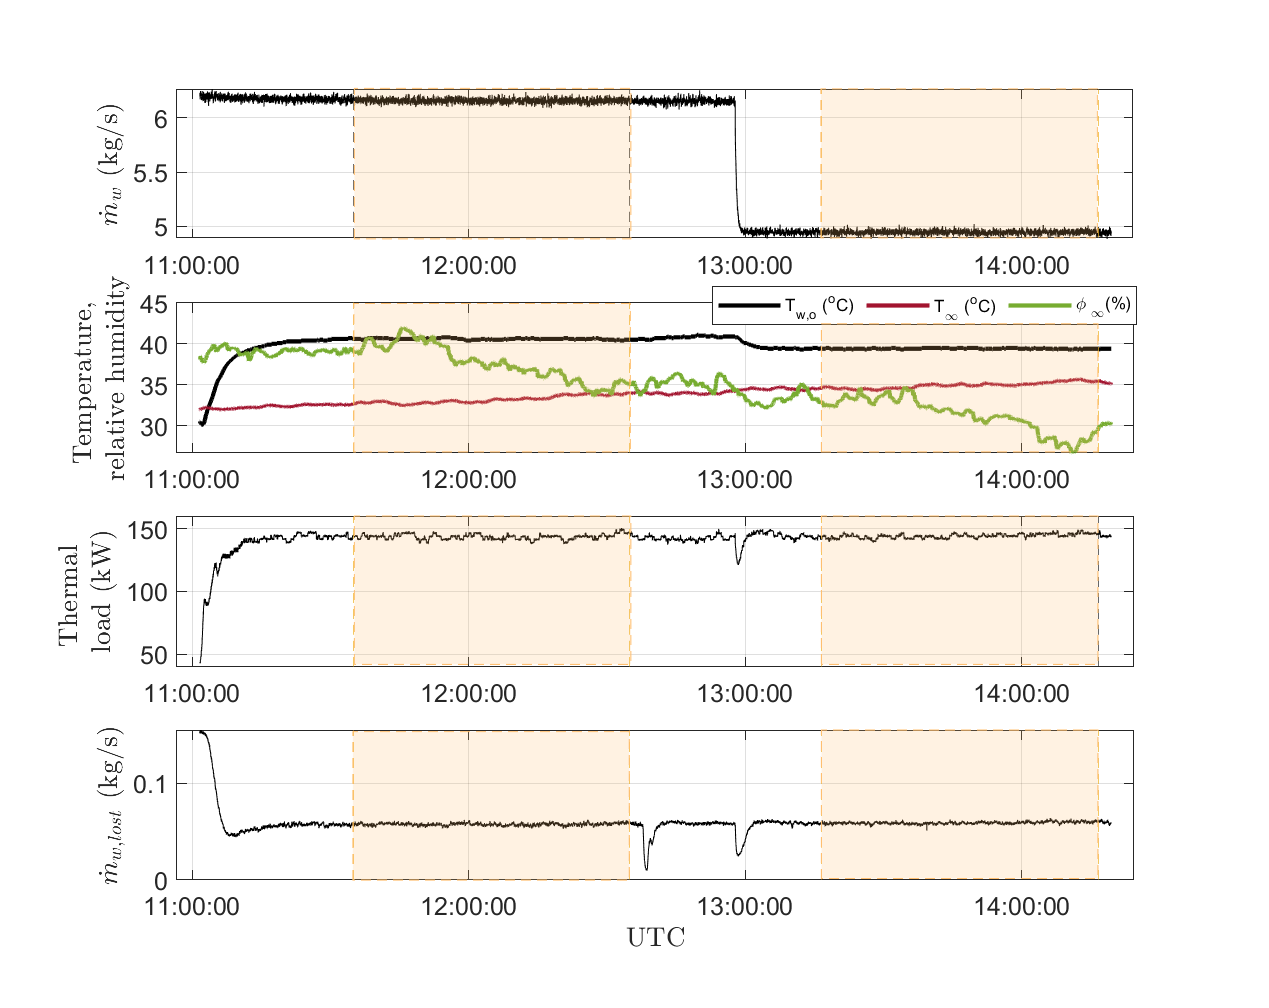
\includegraphics[]{figures/wascop-test-220726.eps}
    \caption{Example of one experiment at the pilot plant in July with two
    valid steady-state operating points.} 
    \labfig{cc:facility:example-test}
\end{figure}

The data from the different experimental campaigns is available at
\sidecite{palenzuela_steadystate_2024a,serrano_wet_2024}.


%===================================
\subsection[Experimental campaign 1]{Experimental campaign 1 -- Exp 1}[Exp 1] 
\labsec{cc:facility:exp:1}

This campaign was specifically designed for the calibration of the physical
model. In total, 19 experimental tests were performed at the combined cooling
pilot plant at PSA. The physical model focuses on the calculation of the
Merkel number which, according to the literature ASHRAE~\sidecite{ashrae_hvac_2004}, is
not a constant value. Instead, it varies depending on the operating
conditions (water-to-air mass flow ratio, $\dot{m}_w/\dot{m}_a$). Therefore,
the experimental campaign has been designed to cover different water-to-air
mass flow ratios. Both variables, the water and the air flow rates, were
varied within the allowable range for plant operation. In the case of the
water flow rate, it ranged from 8 m$^3$/h to 22 m$^3$/h, and in the case of
the air mass flow rate, it was modified by changing the fan frequency from
12.5~Hz to  50~Hz (fan frequency percentage, $f_{fan}$, from 25~\% to
100~\%). The magnitudes required to experimentally determine the air mass
flow rate (air velocity and air temperature and relative humidity) were
measured at the outlet area of the cooling tower\sidenote{Using the sensors
listed in \reftab{cc:facility:instr}}. The outlet area was divided into 9
quadrants and the
above mentioned magnitudes were registered at the center of each quadrant.
The obtained values were averaged to determine the mean velocity, temperature
and relative humidity used in the air mass flow rate calculation. 

Following the same experimental procedure, air velocity,
temperature and humidity maps were measured for 8 different $f_{fan}$ levels
(ranging from 30~\% to 100~\% in 10~\% intervals)\sidenote{This enables to
obtain the air mass flow rate at the outlet of the cooling tower, $\dot{m}_a$,
using the permanent sensors installed in the facility}.

The range of air and water mass flow rates are
1.16-4.32~\mbox{kg/s} and 2.17-6.15~\mbox{kg/s}, respectively. Regarding the
environmental conditions, these were quite similar for all tests in the campaign: high
ambient temperatures (ranging between 32~\mbox{$^\circ$C} and
41~\mbox{$^\circ$C}), and low ambient relative humidities (between
13~\mbox{\%} and 40~\mbox{\%}) since the experiments were carried out during
the summer season.

%===================================
\subsection[Experimental campaign 2]{Experimental campaign 2 -- Exp 2}[Exp 2] 
\labsec{cc:facility:exp:2}

The data required for data-driven models depends on several factors such as the
complexity of the model and the error allowed or the diversity of the inputs.
With the aim of obtaining a reliable model for the WCT, data collected
over several years of operation of the combined cooling system have been used
for tuning. They are a set of 115 stationary data covering the following
operating ranges: ambient temperature, $T_\infty$, \mbox{[9-39] $^{\circ}$C},
ambient humidity, $\phi_\infty$, [10-87] \%, inlet water temperature,
$T_{w,i}$ [33-41] $^\circ$C, cooling water flow rate, $q_w$, [6-23] $m^3/h$
and fan frequency percentage, $f_{fan}$ [21-94]~\%. The thermal load in these
tests varies in the range of [27-178]~${kW}_{th}$. The number of steady-state
data obtained is a reasonable value when compared to other similar data-driven models of
counter-flow cooling towers, as in the case of
\cite{hosoz_performance_2007}, where 81 experimental points
were collected for training and testing.\sidenote{Reminder, dataset is
available at \cite{palenzuela_steadystate_2024a}}

%===================================
\subsection[Experimental campaign 3]{Experimental campaign 3 -- Exp 3}[Exp 3] 
\labsec{cc:facility:exp:3}


With the aim of validating and comparing different modelling approaches, a
dataset of 17 tests (different from the ones taken for experimental campaigns 1
and 2) has been compiled. This experimental campaign was designed using a
design of experiments based on full factorial design with 4 factors and 2
levels (low and high), whose values are shown in
\reftab{cc:facility:exp:3:DoE}.  

\begin{margintable} 
    \caption{Design of experiments for model comparison.} 
    \labtab{cc:facility:exp:3:DoE} 
    % \resizebox{0.5\linewidth}{!}{
    \begin{tabular}{cccc} 
        \toprule Variable & Low level & High level  \\
        \midrule $T_{b}$ ($^{\circ}$C) & $\leq$ 10 & $\geq$ 15 \\
        $T_{w,i}$ ($^{\circ}$C) & $\leq$ 37 & $\geq$ 39 \\
        $\dot{m}_w$ (kg/s) & $\leq$ 3.3 & $\geq$ 5 \\
        $T_{w,i}-T_{w,o}$ ($^{\circ}$C)  & $\leq$ 7 & $\geq$ 8 \\
        \bottomrule 
    \end{tabular}
    % }
\end{margintable}
% \begin{table}[h] 
%     \centering 
%     \caption{Design of experiments for model comparison.} 
%     \labtab{cc:facility:exp:3:DoE} 
%     \resizebox{0.5\linewidth}{!}{
%     \begin{tabular}{cccc} 
%         \toprule Variable & Low level & High level  \\
%         \midrule $T_{b}$ ($^{\circ}$C) & $\leq$ 10 & $\geq$ 15 \\
%         $T_{w,i}$ ($^{\circ}$C) & $\leq$ 37 & $\geq$ 39 \\
%         $\dot{m}_w$ (kg/s) & $\leq$ 3.3 & $\geq$ 5 \\
%         $T_{w,i}-T_{w,o}$ ($^{\circ}$C)  & $\leq$ 7 & $\geq$ 8 \\
%         \bottomrule 
%     \end{tabular}
%     }
% \end{table}

An additional test at design operating conditions of the WCT
(\mbox{$T_{b,\infty}$=21 $^{\circ}$C}, $T_{w,i}$=40 $^{\circ}$C,
$\dot{m}_w$=6.9 kg/s and $T_{w,i}-T_{w,o}$=7 $^{\circ}$C) has been also
included in this test campaign, where $T_{b,\infty}$ is the ambient wet bulb
temperature and $T_{w,o}$ the temperature of the water at the outlet of the
WCT. 


%===================================
%===================================
\subsection{Experimental campaigns for the dry cooler}
\labsec{cc:facility:exp-dc}
